\section{Comparação de substrings de mesmo tamanho}

\begin{frame}[fragile]{Comparação de strings de mesmo tamanho}

    \begin{itemize}
        \item Seja $S$ uma string de tamanho $N$ e considere duas substrings de $S$: 
            $a = S[i..(i + M - 1)]$ e $b = S[j..(j + M - 1)]$, ambas de tamanho $M$

        \item Uma função $f(a, b)$ é uma função de comparação de strings se $f(a, b) < 0$ se
            $a < b$, $f(a, b) = 0$ se $a = b$ e $f(a, b) > 0$ se $a > b$

        \item Usando a comparação caractere a caractere, uma função de comparação pode ser 
            implementada com complexidade $O(M)$

        \item Contudo, uma vez construído o vetor de sufixos $s_A(S)$, esta função pode ser
            implementada em $O(1)$

        \item Para tal, é preciso armazenar os valores das classes de equivalência $cs$ obtidos
            em todas as iterações da construção de $s_A(S)$

        \item Seja $cs[k][i]$ a classe de equivalência da substring cíclica de $S$, de tamanho
            $2^k$, com início na posição $i$
    \end{itemize}

\end{frame}

\begin{frame}[fragile]{Comparação de strings de mesmo tamanho}

    \begin{itemize}
        \item Se $M = 2^k$, então a função $f(a, b)$ corresponde à comparação direta entre
            $cs[k][i]$ e $cs[k][j]$

        \item Caso contrário, $M$ pode ser decomposto em dois blocos de tamanho $2^t$, onde
            $2^t \leq M$ e $2^{t + 1} > M$

        \item O primeiro bloco começa na posição inicial da substring ($i$, no caso da substring
            $a$)

        \item O segundo bloco começa $2^t$ posições antes da última posição (no caso da substring
            $a$, na posição $i + M - 2^t$)

        \item Se as classes de ambas strings em relação ao primeiro bloco são distintas, 
            a comparação entre eles é suficiente

        \item Caso contrário, basta finalizar a comparação utilizando as classes de equivalência
            dos respectivos segundos blocos

        \item Assim, o algoritmo tem complexidade $O(N\log N)$, por conta da construção de 
            $s_A(S)$, e complexidade de memória $O(N\log N)$, por conta da tabela de classes
            de equivalência $cs$
    \end{itemize}

\end{frame}

\begin{frame}[fragile]{Visualização da comparação entre duas substrings de mesmo tamanho}

    \begin{figure}
        \centering

        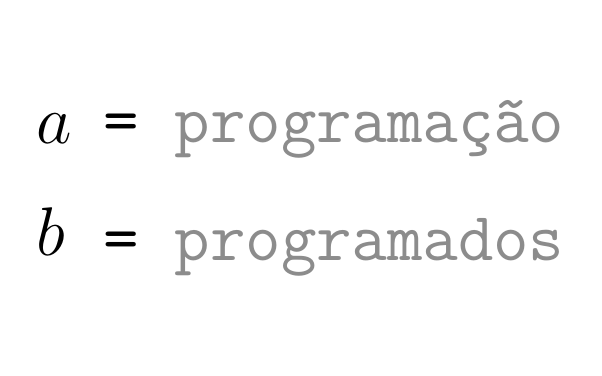
\begin{tikzpicture}
            \node[anchor=west] at (0, 5) { \Huge $a$ };
            \node[anchor=west] at (0.85, 5) { \Huge \texttt{= }\textcolor{gray!90}{\texttt{programação}} };
            \node[anchor=west] at (0, 3.7) { \Huge $b$ };
            \node[anchor=west] at (0.85, 3.5) { \Huge \texttt{= }\textcolor{gray!90}{\texttt{programados}} };
            \draw[opacity=0] (2.0, 5.5) -- (2.0, 5.8) -- node[anchor=south] { $1^o$ bloco } (5.2, 5.8) -- (5.2, 5.5);
            \draw[opacity=0] (2.0, 3.0) -- (2.0, 2.7) -- node[anchor=north] { $1^o$ bloco } (5.2, 2.7) -- (5.2, 3.0);

        \end{tikzpicture}

    \end{figure}

\end{frame}

\begin{frame}[fragile]{Visualização da comparação entre duas substrings de mesmo tamanho}

    \begin{figure}
        \centering

        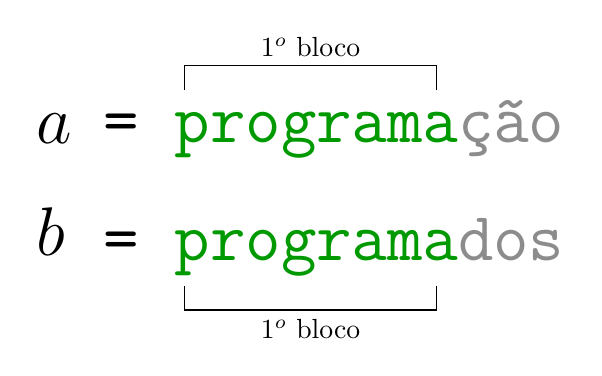
\begin{tikzpicture}
            \node[anchor=west] at (0, 5) { \Huge $a$ };
            \node[anchor=west] at (0.85, 5) { \Huge \texttt{= \textcolor{green!60!black}{programa}\textcolor{gray!90}{ção}} };
            \node[anchor=west] at (0, 3.7) { \Huge $b$ };
            \node[anchor=west] at (0.85, 3.5) { \Huge \texttt{= \textcolor{green!60!black}{programa}\textcolor{gray!90}{dos}} };
            \draw[opacity=1] (2.0, 5.5) -- (2.0, 5.8) -- node[anchor=south] { $1^o$ bloco } (5.2, 5.8) -- (5.2, 5.5);
            \draw[opacity=1] (2.0, 3.0) -- (2.0, 2.7) -- node[anchor=north] { $1^o$ bloco } (5.2, 2.7) -- (5.2, 3.0);

        \end{tikzpicture}

    \end{figure}

\end{frame}

\begin{frame}[fragile]{Visualização da comparação entre duas substrings de mesmo tamanho}

    \begin{figure}
        \centering

        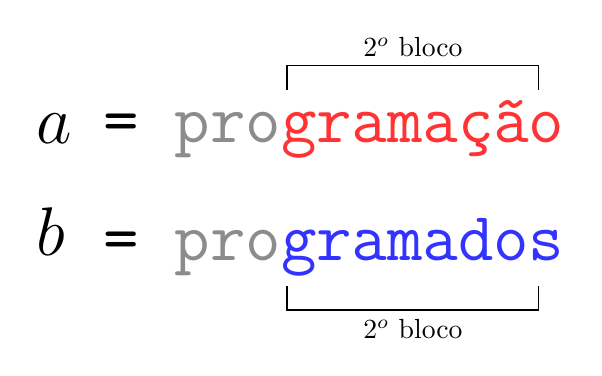
\begin{tikzpicture}
            \node[anchor=west] at (0, 5) { \Huge $a$ };
            \node[anchor=west] at (0.85, 5) { \Huge \texttt{= \textcolor{gray!90}{pro}\textcolor{red!80}{gramação}} };
            \node[anchor=west] at (0, 3.7) { \Huge $b$ };
            \node[anchor=west] at (0.85, 3.5) { \Huge \texttt{= \textcolor{gray!90}{pro}\textcolor{blue!80}{gramados}} };
            \draw[opacity=1] (3.3, 5.5) -- (3.3, 5.8) -- node[anchor=south] { $2^o$ bloco } (6.5, 5.8) -- (6.5, 5.5);
            \draw[opacity=1] (3.3, 3.0) -- (3.3, 2.7) -- node[anchor=north] { $2^o$ bloco } (6.5, 2.7) -- (6.5, 3.0);

        \end{tikzpicture}

    \end{figure}

\end{frame}

\begin{frame}[fragile]{Implementação da comparação de substrings de mesmo tamanho em $O(1)$}
    \inputsnippet{cpp}{88}{99}{substrings.cpp}
\end{frame}
